% TODO (but maybe not here?): explain why and how we define our own meta schema based on json schema, because we use just subset of its features and because our schema is used to generate schema editor GUI and therefore should only show what is supported. Also we want to add descriptions and maybe more. Also limit options to not overwhelm and confuse the user.
% TODO also describe more the users perspective how users would use the tool?

% felix
\subsection{Overview}\label{subsec:overview} % todo maybe rename it requirements?
Before we dive into the architecture and detailed design of the tool, this section provides an overview of the tool from the view of the user.

Figure \ref{mockup_gui_config} provides a sketch of the intended user interface design, showing the \textbf{file editor mode}. 

The application is divided into two main panels: the  \textbf{Text editor panel} (on the left) and the \textbf{GUI editor panel} (on the right).
In the Text editor panel the user can modify their data by hand, just like in a regular text editor. 
On top of that, features like syntax highlighting and schema validation assist the user.
In the GUI editor panel, the user can modify their data with the help of a GUI. 
This GUI is based on the schema which the user provides (more on that in the next paragraphs). 
For enum properties, the user will get a dropdown menu with the different options to choose from, for boolean properties the user will get a checkbox and so on. 
Other features, such as tooltips that display the description and constraints of a property, further assist the user.

This design combines the benefits of both a rich text editor (very efficient for many tasks, more suited for users with technical understanding of the data structure) with the benefits of a GUI (enables users without deep technical understanding to work with the data, assists also expert users).


\begin{figure*}[!t]
    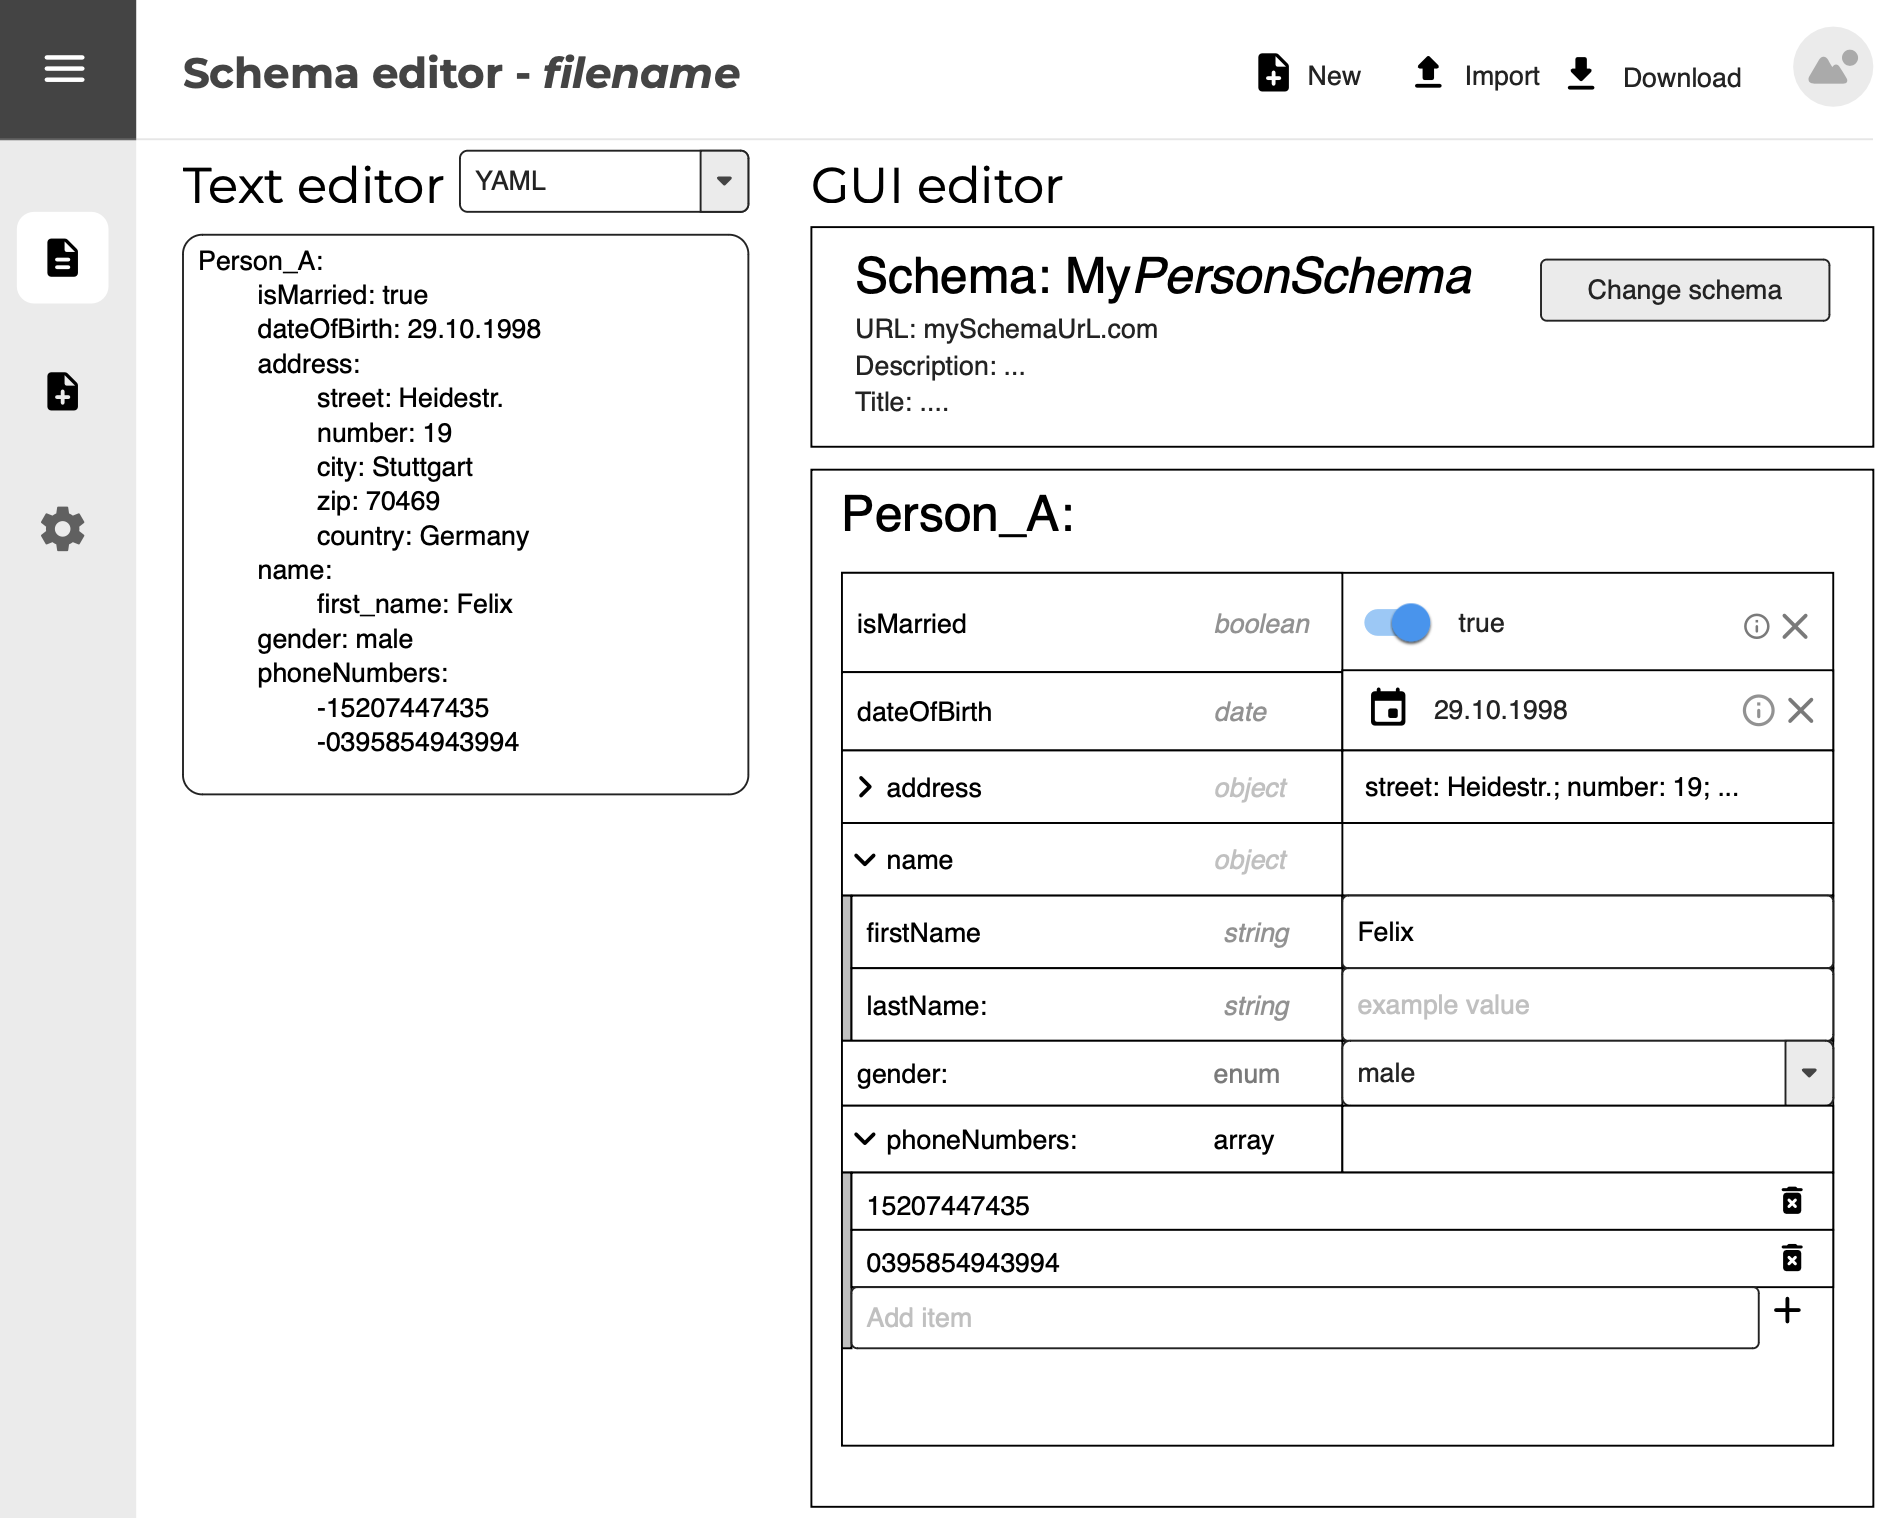
\includegraphics[width=\textwidth]{figures/mockup_gui_config}
    \caption{Sketch of the Tool. File Editor view.}
    \label{mockup_gui_config}
\end{figure*}

% TODO: add numbered annotations to the screenshot and explain them here
%\begin{enumerate}
%    \item Blabla this is the menu bar
%\end{enumerate}


Besides editing their data with the tool, the user can also use it to modify their schema or create a new schema.
This is illustrated in figure \ref{mockup_gui_schema} which sketches the \textbf{schema editor mode}.
The structure of the user interface remains the same as in the file editor mode.
The main difference in this mode is, that the schema being used for the GUI and schema validation is not a user schema, but instead the JSON schema meta schema itself. 

The exemplary file editor tab sketch in figure \ref{mockup_gui_config} shows user data based on a schema called \textit{ArchitectureSchema}.
This \textit{ArchitectureSchema} is shown from the schema editor tab perspective in figure \ref{mockup_gui_schema}.

\begin{figure*}[!t]
    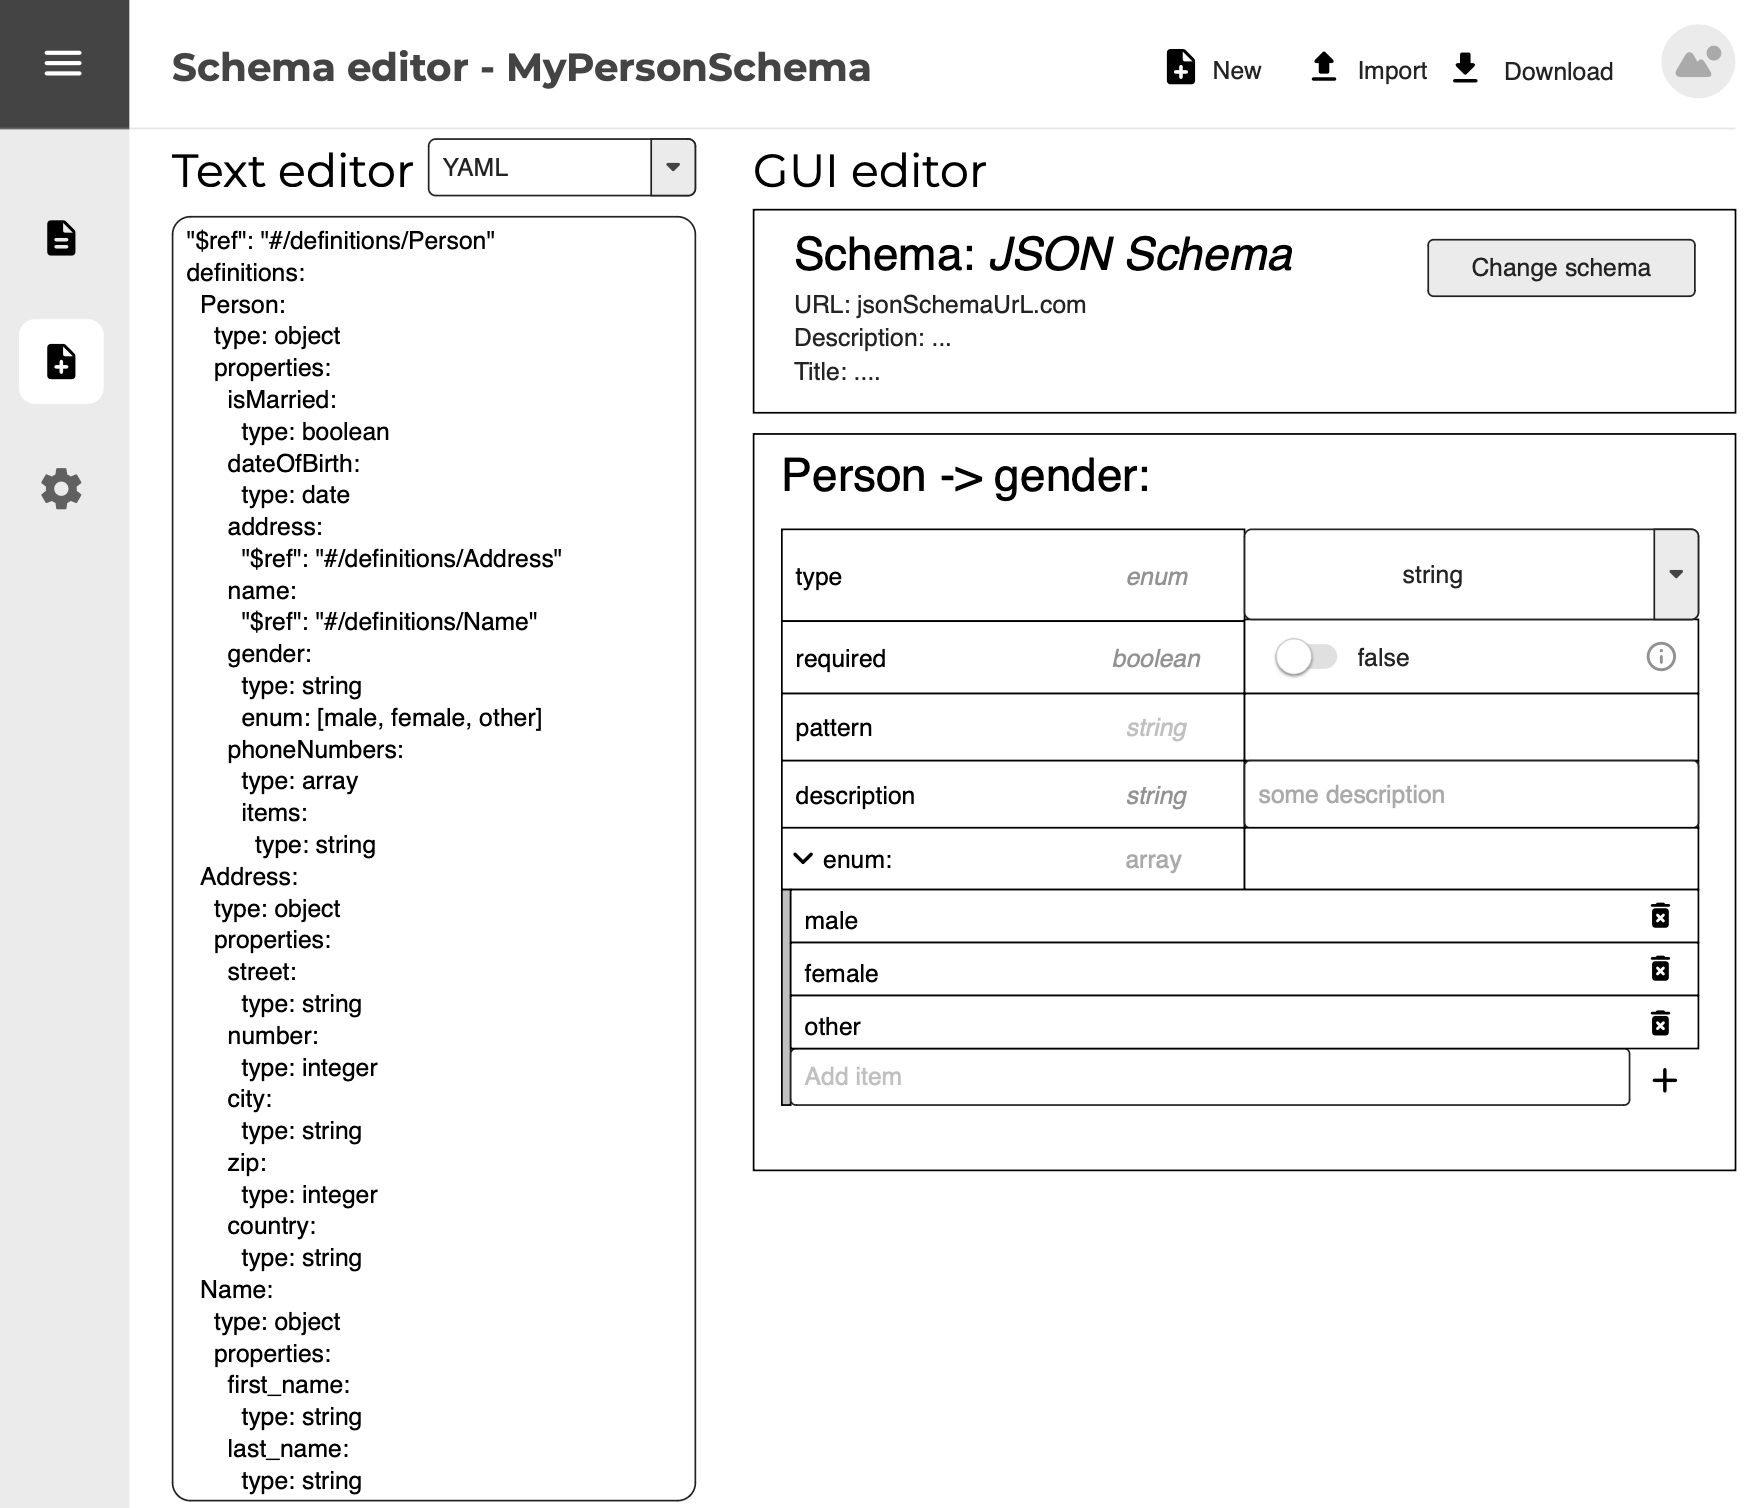
\includegraphics[width=\textwidth]{figures/mockup_gui_schema}
    \caption{Sketch of the Tool. Schema Editor view.}
    \label{mockup_gui_schema}
\end{figure*}

As a schema is a \cfgfile{} itself, it can be treated as such and the tool can offer assistance accordingly.
Note that whenever the user edits a \cfgfile{} using the tool, they do so using some underlying schema.
Even the tool settings can be seen as a \cfgfile{}, for which the underlying schema is a settings schema.
%When editing a schema file, the underlying schema will be the schema of JSON Schema.
Table \ref{tab:schema_and_file_data_by_mode} illustrates how for the different modes, file data and schema being used by the tool differ.
\begin{table}[!t]
\caption{File data and schema for the different modes}
\label{tab:schema_and_file_data_by_mode}
\centering
\begin{tabular}{lll}
\toprule
\textbf{Mode} & \textbf{Effective File Data} & \textbf{Effective Schema} \\ 
\midrule
File editor   & User data                    & User schema               \\
Schema editor & User schema                  & JSON Meta Schema          \\
Settings      & Settings data                & Settings schema           \\
\bottomrule
\end{tabular}
\end{table}



% felix

\subsection{Architecture}\label{subsec:architecture} % todo diagram illustrating the architecture
% todo mention that its frontend only
The core of our tool is a single source of truth data store that contains the current user configuration data (as a JavaScript Object).
With this data store we can bidirectionally connect what we call ``editor panels''.
An editor panel is a modular component that the user of the tool can access to modify the config data in an indirect way.
It might be implemented as a raw text editor, a graphical user interface or any other way in which the data can be presented to the user.
All editor panels are independent and do only have access to the data store but not to each other.
Every editor panel subscribes to the changes of the data store, so it can be updated accordingly whenever the data in the store is changed.
Additionally, every panel has the capabilities of updating the data store themselves, which is done when the user modifies the data in the editor panel.
The following example use-cases illustrate the capabilities of this architecture:

\begin{itemize}
    \item Format converter: one panel shows the data in a rich-text editor in JSON format, a second panel shows the data in a rich-text editor in YAML format. Any semantic data change on one panel will cause the same semantic change in the other panel.
    \item Split-Screen Editor: one panel shows the data in a rich-text editor, a second panel shows the data in a GUI. This way the user can have the efficiency of a text editor, but also the assistance of a GUI at the same time. Any semantic data change on one panel will be forwarded to the other panel. The GUI editor panel would require some data schema.
    \item The Split-Screen Editor could be implemented for different data formats, such as YAML, JSON and XML. The architecture allows any data format as long as there exists a mapping from this data format to a JavaScript Object and back.
\end{itemize}

% TODO: Add diagram with store in center in several panels with bidirectional connection of subscribe/update

% felix

\subsubsection{Single Source of Truth Data Store}
this is the core of the tool.
The panels can subscribe to this store to receive updates whenever data is changed.
Also, panels can trigger changes of the data in the store.
Besides the current configuration data, the store also stores the \textit{path of the currently selected data entry} and the schema that is currently being used.

% felix

\subsubsection{Text Editor Panel} % todo instead of writing in future, write in simple present
For the text editor panels, we embed a rich-text editor that already supports syntax highlighting and other useful features.
We enable validation of whether the text is well-formed according to the JSON/YAML/XML Standard and add schema validation.
The architecture allows for having one text editor panel that supports multiple languages, as well as for having separate text editor panels, one for each language.
The panels subscribe to the data store.
Whenever the configuration data is changed in the store, the panels will take the new configuration data JavaScript Object, serialize it into the given language and replace the text in the text editor with the new serialized data.
The action of replacing the text in the text editor will cause formatting and comments to be lost.
An alternative to replacing the complete text in the text editor, whenever data in the store is changed, would be to only replace the section of the text, which corresponds to the change.
This would require on the one hand identifying which part of the data is affected by the change and on the other hand understanding of the data within the serialized text in a way that it can be manipulated (e.g.\ navigating within the hierarchical data structure and changing values of a given path). 
This is out of scope for the project, but may be part of future work.
Even such deep understanding of the text would wipe out non-default formatting at the sections affected by change.
We tackle those difficulties in the following way: we accept that user-specific text formatting might be undone by our tool.
To allow for different styles of formatting, we will provide the user with global formatting style settings (such as level of indentation or whether in YAML strings should be in quotation marks or not). % todo actually implement this
Whenever the configuration data JavaScript Object is serialized into text, we apply those formatting style settings.
Second, to deal with the loss of comments, we implement a technique that keeps track of any comments in the text and then restores them after the text is replaced. % todo either write that we don't support it for now or implement it

When the user edits the text in the text editor, the text is deserialized into a JavaScript Object and sent to the data store, which then updates the configuration data object and notifies all other subscribed panels of the change.

To make it possible to highlight certain lines in the editor as erroneous (schema violations) or jump to certain lines (e.g. when the user selects a property in the GUI editor, we want to jump to the same property in the text editor), we need a function \textit{determineRow(editorContent, dataPath)} that can determine the corresponding editor line, based on the configuration text and a given data path. See listing \ref{listing:determineRow} for an example input and output of such a function.

\begin{listing}[!h]
    \begin{minted}[frame=single,
        framesep=3mm,
        linenos=true,
        xleftmargin=15pt,
        tabsize=4]{js}
editorContent = 
  "{
     'people':
       [
         { 
           'age': 22, 
           'name': 'alex' 
         },
         { 
           'age': 5, 
           'name': 'bola' 
         }
       ]
   }";
   
resultRow1 = determineRow(
	editorContent,
	"people"
 );
 # resultRow1 = 1 
 
resultRow2 = determineRow(
	editorContent,
	"people.0.age"
 );
 # resultRow2 = 4
 
resultRow3 = determineRow(
	editorContent,
	"people.1.name"
 );
 # resultRow3 = 9
 
    \end{minted}
    \caption{Example input and output for \textit{determineRow(editorContent, dataPath)}}
    \label{listing:determineRow}
\end{listing}

The other way around, when the user places their cursor inside the text editor, we want to determine the path of the element that the cursor is currently at. This requires a function \textit{determinePath(editorContent, cursorPosition)} which returns a data path based on the configuration text and a given cursor position.

For the tool to support a data format, such as JSON, YAML or XML, the following needs to be implemented for that format:
\begin{itemize}
	\item Function to stringify a JavaScript object to a string in the data format
	\item Function to parse a string in that data format as a JavaScript object
	\item determineRow(editorContent, dataPath) 
	\item determinePath(editorContent, cursorPosition)
\end{itemize}

% felix

\subsubsection{GUI Assistance Panel}
The GUI assistance panel(s) directly work with the given schema and provide the user with corresponding GUI elements, such as a checkbox for a boolean data structure or a text field for a string data structure.
Additional GUI elements, such as tooltips (showing the description of a data field) are used to support the easier.
The GUI elements are constructed in the following manner: a schema is seen as a hierarchical tree of data field definitions and their corresponding constraints.
A data field can either be simple (string, boolean, number, \ldots) or complex (array or dictionary of data fields).
Every schema has a root data field.
The GUI element for this root data field is constructed. % todo describe tree generation
When constructing the GUI element for a complex data field, this includes constructing the GUI elements for all child data fields too.
This way, the whole schema tree is traversed and GUI elements for all entries are constructed.
To avoid overwhelming the user with too many GUI elements, the ones with child elements can be expanded or collapsed by the user and only a limited amount of them is expanded by default.
By design, each of these constructed GUI elements is mapped to their corresponding data field (in other words: to a path in the data structure).
The initial values of all GUI elements are taken from the data in the store, by accessing the data at the given paths.
Whenever the values in a GUI element are adjusted by the user, the data in the store will be updated with the new values.


%In the following, the corresponding GUI elements for the different JSON Schema data types and constraints are shown:
%
%\textbf{Boolean}
% todo: describe how it works. Then also describe for all the different data types, how we intend to implement the GUI aspect. E.g. for boolean we have checkbox